\section{Experiments}

\subsection{Experiment 1:}
\subsection{Experiment 2: Logical and Physical Optimization Impact}

This experiment evaluates the effectiveness of the logical and physical optimization strategies adopted by \textsc{GALOIS}, following the methodology described in Sections~4 and~5 of the original paper. 
The goal is to isolate and quantify how different execution strategies affect result quality, measured through the \textbf{AVG-Score} (average of F1-Cell, Cardinality, and Tuple Constraint).

\vspace{0.5em}
\noindent
All experiments are conducted on the \textbf{GEO} dataset, which queries the internal parametric knowledge of the LLM and includes 32 SQL queries with pre-computed ground truth.

\paragraph{Physical Optimization.}
At the physical level, \textsc{GALOIS} selects how data is retrieved from the LLM. 
For each query, we compare three execution strategies:
\begin{itemize}
    \item \textbf{Table-Scan}: retrieves full tuples in a single scan, providing broader context to the LLM.
    \item \textbf{Key-Scan}: first retrieves key values and then populates remaining attributes, using a chain-of-thought style interaction.
    \item \textbf{AUTO}: lets \textsc{GALOIS} automatically choose between Table-Scan and Key-Scan based on the confidence estimator described in the paper.
\end{itemize}

We report both the average result quality and the total token consumption. 
Additionally, we evaluate the \emph{AUTO accuracy}, i.e., how often the automatically selected strategy matches the best-performing fixed strategy (Table-Scan or Key-Scan) for a given query.

\begin{table}[ht]
    \centering
    \caption{Physical optimization results on GEO (AVG-Score and token usage).}
    \label{tab:exp2-physical}
    \resizebox{0.75\textwidth}{!}{
    \begin{tabular}{lcc}
        \toprule
        \textbf{Strategy} & \textbf{AVG-Score} & \textbf{Tokens (M)} \\
        \midrule
        Table-Scan & \textbf{0.315} & 0.030 \\
        Key-Scan   & 0.272 & 0.033 \\
        AUTO       & 0.274 & 0.031 \\
        \bottomrule
    \end{tabular}}
\end{table}

The results show that, on GEO, \textbf{Table-Scan achieves the highest average quality}, suggesting that richer contextual prompts help the LLM retrieve more complete and accurate data.
The AUTO strategy closely follows the best fixed plan, confirming that the confidence-based physical planner behaves robustly, although the gain over Table-Scan is limited for this dataset.

\paragraph{Logical Optimization.}
To isolate the impact of logical planning decisions, we fix the physical strategy to \textbf{Table-Scan} and evaluate different predicate pushdown strategies, as described in the paper:
\begin{itemize}
    \item \textbf{NO-PUSH}: no conditions are pushed down into the LLMScan.
    \item \textbf{PUSH-ALL} (\textsc{GALOIS\textsubscript{A}}): all WHERE conditions are pushed down.
    \item \textbf{PUSH-CONFIDENT} (\textsc{GALOIS\textsubscript{F}}): only conditions selected by the confidence estimator are pushed down.
\end{itemize}

Only queries with at least two WHERE conditions are considered, in accordance with the experimental protocol of the original work.

\begin{table}[ht]
    \centering
    \caption{Logical optimization results on GEO with fixed Table-Scan.}
    \label{tab:exp2-logical}
    \resizebox{0.75\textwidth}{!}{
    \begin{tabular}{lcc}
        \toprule
        \textbf{Strategy} & \textbf{AVG-Score} & \textbf{Tokens (M)} \\
        \midrule
        NO-PUSH                 & 0.318 & 0.015 \\
        GALOIS A (push all)     & 0.274 & 0.009 \\
        GALOIS F (confident)   & \textbf{0.397} & 0.014 \\
        \bottomrule
    \end{tabular}}
\end{table}

The results clearly show that \textbf{confidence-based pushdown (\textsc{GALOIS\textsubscript{F}})} significantly outperforms both NO-PUSH and PUSH-ALL strategies.
This confirms the key intuition of the paper: pushing all predicates may reduce cost but often degrades result quality due to increased reasoning complexity for the LLM, while selectively pushing only confident predicates yields a better balance between precision and recall.

\paragraph{Comparison with the Paper.}
Our findings are fully consistent with the original GALOIS results.
In particular, we observe the same qualitative trends:
\begin{itemize}
\item \textbf{(i)} Table-Scan can outperform Key-Scan when additional context improves factual retrieval, and
\item \textbf{(ii)} confidence-driven logical optimization (\textsc{GALOIS\textsubscript{F}}) consistently achieves the best AVG-Score among logical strategies.
\end{itemize}
These results further validate the robustness of the GALOIS optimization framework across datasets and implementations.


\subsection{Experiment 3:}
\subsection{Experiment 4:}

Here we implemented an automated evaluation pipeline  ("Impact of Rarity and Temporality"), focusing on the \textbf{PRESIDENTS} domain. The primary objective is to quantify how the frequency of data in pre-training (popularity) and its temporal recency influence the ability of Large Language Models (LLMs)  to measure two specific biases.
\begin{itemize}
    \item \textbf{Rarity}: Compares performance on popular entities (USA) versus rare entities (Venezuela).
    \item \textbf{Temporality}: Compares performance on recent events versus historical events . For this purpose we split the queries into three categories: ALL-TIME covering all dates, RECENT for queries that cover data from late 1900 to today, and PAST for queries
for data till the late 1900.
\end{itemize}



By benchmarking model modalities (GALOIS, NL, SQL) against the Ground Truth, the script calculates the AVG-SCORE. The results confirm that query generation quality degrades significantly when dealing with rare or historical data, as we can see in the tables below:

\begin{table}[ht]
    \centering
    \caption{Experimental Results: Impact of Rarity and Temporality on Query Execution Quality (AVG-SCORE).}
    \label{tab:combined_results}
    \begin{tabular}{lcccccc}
        \toprule
        \textbf{Category} & \textbf{GALOIS\textsubscript{A}} & \textbf{GALOIS\textsubscript{F}} & \textbf{GALOIS\textsubscript{S}} & \textbf{GALOIS\textsubscript{WO}} & \textbf{NL} & \textbf{SQL} \\
        \midrule
        \multicolumn{7}{l}{\textit{Impact of Rarity (Country)}} \\
        \midrule
        Presidents-USA & 0.570 & \textbf{0.652} & 0.587 & 0.089 & 0.352 & 0.320 \\
        Presidents-Venezuela & 0.282 & 0.212 & \textbf{0.323} & 0.051 & 0.091 & 0.257 \\
        \midrule
        \multicolumn{7}{l}{\textit{Impact of Temporality}} \\
        \midrule
        Recent & \textbf{0.532} & 0.531 & 0.449 & 0.095 & 0.375 & 0.318 \\
        Past & 0.240 & 0.305 & \textbf{0.378} & 0.000 & 0.183 & 0.281 \\
        All-Time & 0.427 & 0.420 & \textbf{0.479} & 0.077 & 0.160 & 0.277 \\
        \bottomrule
    \end{tabular}
\end{table}


\subsection{Experiment 5: Impact of SQL Query Complexity on Retrieval Quality}
\textbf{Objective}: The objective of this experiment is to evaluate the robustness and stability of the GALOIS system as the structural and logical complexity of the input SQL query varies. Since Large Language Models (LLMs) tend to degrade in performance when handling complex logic (such as multiple joins or nested aggregations).
\\\textbf{Methodology and Query Taxonomy}: To conduct this analysis, we implemented a static classifier (\texttt{classify\_query\_complexity}) that parses the Abstract Syntax Tree (AST) of each SQL query via \texttt{sqlglot} and assigns it to one of six mutually exclusive complexity categories, ordered by expected difficulty:
\begin{itemize}
    \item \textbf{SP2 (Selection-Projection Simple)}: Linear queries involving only selection and projection operations with at most 2 conditions in the \texttt{WHERE} clause. These represent the simplest base case.
    \item \textbf{SP2> (Selection-Projection Complex)}: Selection/projection queries featuring more than 2 filtering conditions, requiring the LLM to manage a denser logical context.
    \item \textbf{DIST (Distinct)}: Queries including the DISTINCT clause, requiring the system to handle explicit result deduplication.
    \item \textbf{AGGR (Aggregation)}: Queries utilizing aggregation functions (COUNT, SUM, AVG, MAX, MIN), which require arithmetic reasoning or counting capabilities on retrieved tuples.
    \item \textbf{G/O (Group By / Order By)}: Queries imposing sorting or grouping of data, testing the system's ability to structure output sequentially.
    \item \textbf{JOIN}: Queries involving joins between two or more tables. This is considered the most complex category, as it requires the system to decompose the problem into multiple scans (multi-table retrieval) and reconstruct relationships in local post-processing.
\end{itemize}
The GALOIS results are compared against the Ground Truth (loaded from pre-calculated JSON files) using three metrics: F1-Cell Exact, Cardinality, and Tuple Constraint of the \texttt{galois\_eval.py} script.
In Figure \ref{fig:exp5-avg} we compare metrics of our run with the GALOIS paper ones and is clear that JOIN operations are worsening the results.
The main reason for that is the difficulty of LLM to retrieve results that match the queries with JOIN clause, something already seen in the GALOIS results in Section \ref{results_galois}.

\begin{figure}[H]
    \centering
    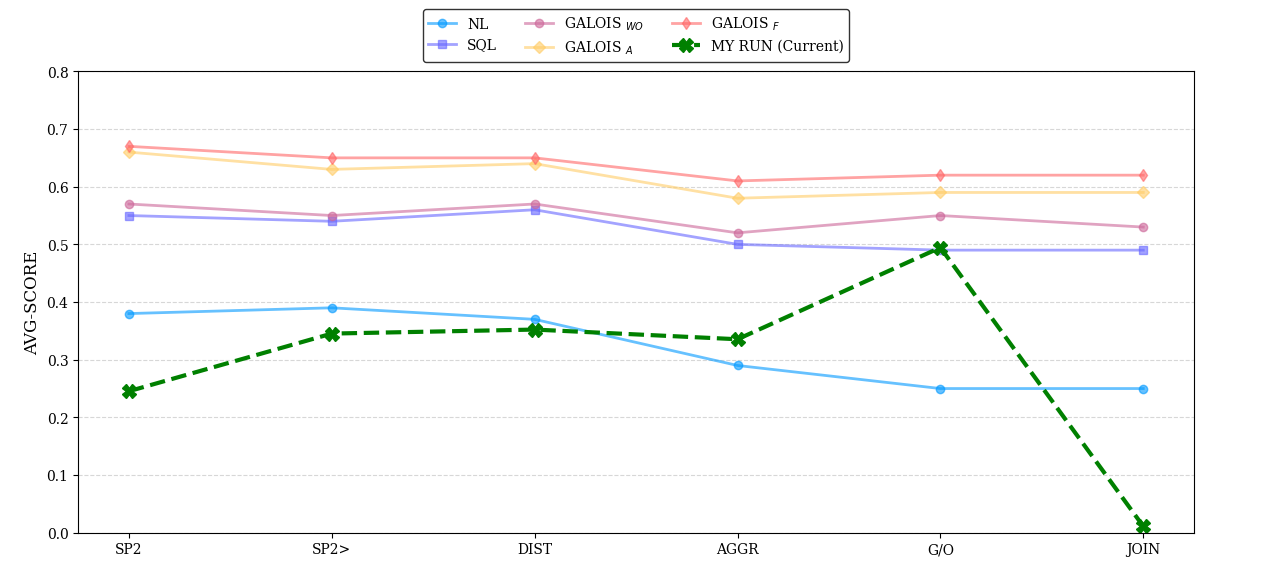
\includegraphics[width=0.9\textwidth]{images/exp-5-avg.png}
    \caption{Result quality w.r.t query complexity}
    \label{fig:exp5-avg}
\end{figure}






\subsection{Experiment 6:}
\subsection{Experiment 7:}
\subsection{Experiment 8:}
\textbf{Objective}: This experiment aims to quantify the efficacy of the \textbf{Logical Planner} (the component deciding which strategy to adopt) by measuring the "Optimality Gap". The Optimality Gap represents the performance difference between the automatic choice made by \texttt{GALOIS\_F} and the theoretical optimal choice ("Oracle") that the system could have made if it had selected the best possible strategy for every single query.
For every query present in the target datasets (GEO, WORLD, MOVIES), the runner  executes the configurations in "brute-force" mode.
\\\textbf{Oracle Definition and Gap Calculation}: For each query $q$, we define the Oracle score ($S_{opt}$) as the maximum score obtainable among the available strategies:$$S_{opt}(q) = \max(S_{GALOIS\_A}(q), S_{GALOIS\_WO}(q), S_{GALOIS\_F}(q))$$.\\ \textbf{The Optimality Gap} is calculated as the average difference between the Oracle and the adaptive variant:$$Gap = \frac{1}{N} \sum_{q \in Q} (S_{opt}(q) - S_{GALOIS\_F}(q))$$ A gap close to 0 indicates that the GALOIS\_F automatic selector is choosing the best available strategy almost every time. A high gap suggests that, although a winning strategy exists for that query (e.g., Key-Scan), the system erroneously opted for another
Results in Figure \ref{fig:exp8} report the AVG-Score on All the queries in the dataset, and we also break the AVG-Score for each dataset.

\begin{figure}[H]
    \centering
    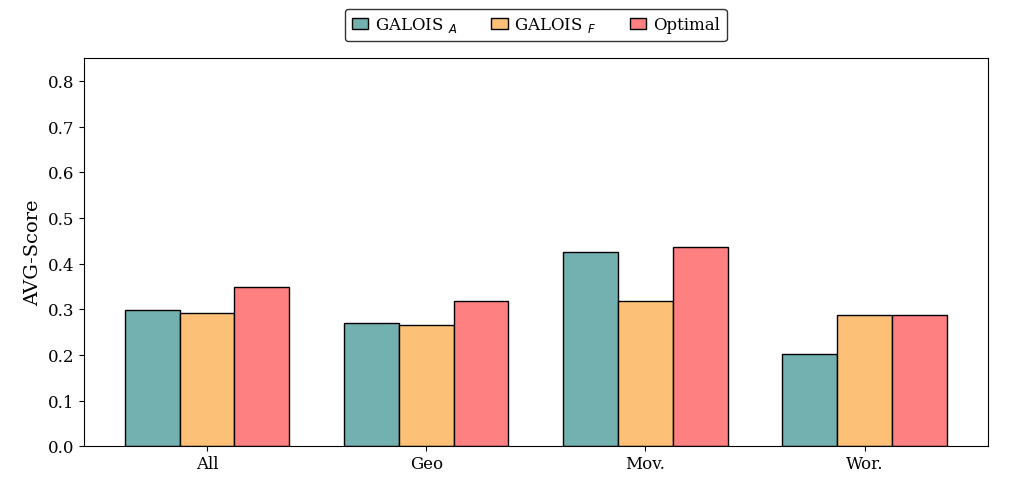
\includegraphics[width=0.9\textwidth]{images/exp-8.png}
    \caption{AVG-Score Comparison for Galois A and Galois F against the optimal plans across all datasets.}
    \label{fig:exp8}
\end{figure}